% !TEX encoding = UTF-8 Unicode
\documentclass[11pt, a4paper, titlepage, portuguese]{article}
\usepackage[]{geometry}
	\geometry{
		a4paper,
		includehead,
		includefoot,
		top=1.7cm,
		bottom=1.7cm,
		left=2.5cm,
		right=2.5cm
	}
%\usepackage{fontspec} % XeLaTeX
\usepackage[T1]{fontenc} % LaTeX
\usepackage[utf8]{inputenc} % LaTeX
%\usepackage{newtxmath, newtxtext}
\usepackage{csquotes}
\usepackage{babel}
%\usepackage[backend=bibtex]{biblatex}
%\usepackage[backend=biber]{biblatex}
%\addbibresource{bibliography.bib}

\usepackage{indentfirst}
\usepackage{graphicx}
	\graphicspath{{images/}}
\usepackage{grffile}
\usepackage{float}
\usepackage{amsmath}
	\allowdisplaybreaks
\usepackage{physics}
\usepackage{siunitx}
	\sisetup{inter-unit-product =\ensuremath{.}}
\usepackage{hyperref}

% Section styles
%\renewcommand{\thesection}{\Roman{section}}
%\renewcommand{\thesubsection}{\alph{subsection})}
%\renewcommand{\thesubsubsection}{\roman{subsubsection}.}

% Useful commands
\newcommand{\eq}{\Leftrightarrow} % Equivalente
% Ordem de grandeza, e.g., "2\og{5}" => "2e5"
\newcommand{\og}[1]{{\times \num{e#1}}}
% Para numerar apenas uma equação
\newcommand\numberthis{\addtocounter{equation}{1}\tag{\theequation}}

% Header and footer
\usepackage{fancyhdr}
\pagestyle{fancy}
\fancyhf{}
\lhead{Electrotecnia Teórica}
\rhead{1º Laboratório}
\lfoot{IST - Engenharia Eletrotécnica e de Computadores}
\rfoot{Página \thepage}
\renewcommand{\headrulewidth}{1pt}
\renewcommand{\footrulewidth}{0.5pt}

% Document
\begin{document}
	\begin{titlepage}
		\center
		\textsc{\bfseries\huge Instituto Superior Técnico}\\[1cm] % Name of your university/college
		\includegraphics[height=2cm]{IST_Logo.pdf}\\[2.5cm]

		\textsc{\Large Engenharia Eletrotécnica e de Computadores}\\[0.5cm] % Major heading such as course name
		\textsc{\bfseries{\LARGE Eletrotecnia Teórica}}\\[0.5cm] % Minor heading such as course title
		\textsc{\Large 2017/2018 2º Semestre}\\[1.5cm]

		\rule{\textwidth}{1.6pt}\vspace*{-\baselineskip}\vspace*{2pt} % Thick horizontal line
		\rule{\textwidth}{0.4pt}\\[\baselineskip] % Thin horizontal line
			\textsc{\Huge \bfseries 1º Trabalho Laboratorial}\\[0.2cm]
			\bigskip
			\textsc{\Large \bfseries Determinação Experimental Da Matriz De Coeficientes De Capacidade De Um Sistema De N+1 Condutores \\
			(Via Analogia Reo-eléctrica)}\\[0.2cm]
		\rule{\textwidth}{0.4pt}\vspace*{-\baselineskip}\vspace{3.2pt} % Thin horizontal line
		\rule{\textwidth}{1.6pt}\\[5cm]

		\begin{minipage}{0.9\textwidth}
			\begin{flushleft} \large
				\begin{Large}\bfseries\textsc{Autores:}\end{Large}\\[0.4cm]
				\begin{tabular}{l l l}
					Ricardo Simões			& 70389 & \normalsize ricardo.f.d.simoes@ist.utl.pt \\
					Rita Ramos					& 81616 & \normalsize rita.ramos@tecnico.ulisboa.pt \\
					João Pinheiro				& 84086 & \normalsize joao.castro.pinheiro@tecnico.ulisboa.pt \\
					João Sebastião			& 84087 & \normalsize joaofpsebastiao@tecnico.ulisboa.pt \\
				\end{tabular}
			\end{flushleft}
		\end{minipage}\\[0.5cm]

		\large \bfseries Laboratório segunda-feira, 09h30-11h30, Grupo D\\
		\large 12 de março de 2018\\[1cm]
		\setcounter{page}{0}
	\end{titlepage}
	%\tableofcontents

	\section{Dimensionamento}
	\subsection{a)}

		\par
		Admitindo que a água é um meio linear, ou seja, $\vec{J} = \sigma \vec{E}$ e que $\vec{E}$ e $\vec{J}$ são uniformes dentro do tanque, dado que $\vec{J} // \vec{n}$, então:

		$$ U = RI \eq R = \dfrac{U}{I} = \dfrac{\int\limits_{\text{placa}(4)}^{\text{placa}(0)} \vec{E} \vdot \dd{\vec{s}}}{\int\limits_{S_{(4)}}(\vec{J} \vdot \vec{n})\dd{S}} = \dfrac{aE}{\sigma Ewl} = \dfrac{a}{\sigma wl}$$
		\par
		Para determinar experimentalmente a condutividade da água ($\sigma$) , é necessário medir $U$ e $I$, obtendo assim a expressão:

		$$ R = \frac{U}{I} = \dfrac{a}{\sigma wl} \eq \sigma = \frac{I}{U} \dfrac{a}{wl}$$

	\subsection{b)}

	\par
	Segundo a analogia reo-elétrica, é possível estabelecer uma relação entre a capacidade de um condensador e a condutância elétrica quando a geometria dos dois sistemas a comparar é idêntica.
	Sabe-se que na presença de uma corrente estacionária, a intensidade de corrente é dada por:

	\begin{align*}
		\int_S \vec{J} \vdot \vec{n}\dd{S} = I
	\end{align*}

	\par
	Na situação do ensaio da figura 2, a intensidade do campo elétrico é constante e este é paralelo à normal, obtendo assim:

	\begin{align*}
		\vec{J} = \sigma \vec{E} \Rightarrow \int_S \vec{J} \vdot \vec{n} \dd{S} = \int_S \sigma \vec{E} \vdot \vec{n} \dd{S}  = \sigma E S = I
	\end{align*}

	\par
	Na presença de um campo elétrico estático, pela aplicação da Lei de Gauss, tem-se:

	\begin{align*}
			\int_S \vec{D} \vdot \vec{n} \dd{S} = Q
	\end{align*}

	\par
	Do mesmo modo, devido ao facto de a intensidade do campo elétrico ser constante e paralelo à normal, tem-se:

	\begin{align*}
		\vec{J} = \epsilon \vec{E} \Rightarrow \int_S \vec{D} \vdot \vec{n} \dd{S} = \int_S \epsilon \vec{E} \vdot \vec{n} \dd{S} = \epsilon E S = Q
	\end{align*}

	\par
	Relacionando as expressões da capacidade de um condensador e condutância elétrica com as expressões obtidas acima, obtém-se:

	\begin{align*}
		\begin{cases}
			G = \dfrac{I}{U} = \dfrac{\sigma E S}{U} \\[1em]
    	C = \dfrac{Q}{U} = \dfrac{\epsilon E S}{U}
 		\end{cases}
	\end{align*}

	\begin{align*}
		\Rightarrow &\dfrac{G}{C} = \dfrac{I}{Q} = \dfrac{\sigma}{\epsilon} \Rightarrow Q = I\dfrac{\epsilon}{\sigma}
	\end{align*}

	\begin{figure}[H]
		\centering
		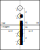
\includegraphics[width=0.4\linewidth]{imagem.pdf}
		\caption{Esquema para o método das imagens}
		\label{fig:imagem}
	\end{figure}

	Recorrendo ao método das imagens, usando a informação presente na \autoref{fig:imagem}, e usando a expressão obtida no laboratório inicial para o cálculo do potencial entre condutores filiformes, tem-se: ERA NECESSÁRIO INCLUIR A DEMONSTRAÇÃO

	\begin{align*}
		V_{ij} = \dfrac{q}{2\pi\epsilon} \ln\left(\dfrac{r'_{ij} }{r_{ij} }\right) = \dfrac{Q}{2\pi\epsilon l} \ln\left(\dfrac{r_{ij} '}{r_{ij} }\right)
	\end{align*}

	\par
	onde $r'_{ij}$ é a distância entre o condutor i e a imagem do condutor j e $r_{ij}$ é a distância real entre os condutores i e j. Por aplicação da Lei de Ohm e fazendo as respetivas substituições, obtém-se finalmente a expressão para calcular os elementos da matriz dos coeficientes de resistência para o sistema de condutores:

	\begin{align*}
		R_{ij} = \dfrac{V_{ij} }{I} = \frac{\dfrac{Q}{2\pi\epsilon l} \ln\left(\dfrac{r'_{ij} }{r_{ij} }\right)}{I}
		= \dfrac{\dfrac{I \epsilon}{2\pi\epsilon \sigma l}}{I} \ln\left(\dfrac{r'_{ij} }{r_{ij} }\right)
		\Rightarrow R_{ij} = \dfrac{1}{2\pi\sigma l}\ln\left(\dfrac{r'_{ij} }{r_{ij} }\right)
	\end{align*}

	\par
	Esta matriz pode ser escrita na forma:

	\begin{align*}
		&[R] = \dfrac{1}{\sigma l} [K]  \\
		&[K] = \dfrac{1}{2 \pi} \ln\left(\dfrac{r'_{ij} }{r_{ij} }\right)
	\end{align*}

	\par
	onde $[K]$ depende apenas raio dos condutores cilíndricos e das distâncias destes entre si e ao plano condutor. Assim, com os dados fornecidos relativamente à posição relativa dos condutores, obtém-se a matriz $[K]$:

	\begin{align*}
		\begin{split}
		[K] &= \dfrac{1}{2\pi}
		\begin{bmatrix}
			\ln\left(\dfrac{2h_1}{r_0}\right) & \ln\left(\dfrac{2h_1 + d}{d}\right)  \\[1em]
			\ln\left(\dfrac{2h_1 + d}{d}\right) & \ln\left(\dfrac{2h_1 + d}{r_0}\right)
		\end{bmatrix} = \\
		&= \begin{bmatrix}
			0.55 & 0.24 \\
			0.23 & 0.62 \\
		\end{bmatrix}
		\end{split}
		\end{align*}

	\subsection{c)}

		\par
		Para calcular a matriz inversa de $[K]$, ou seja $[K]^{-1}$, recorreu-se ao Matlab, obtendo assim:

		\begin{align*}
			[K]^{-1} =
			\begin{bmatrix}
				2.20 & -0.85 \\
  		 -0.86 &  1.94
			\end{bmatrix}
		\end{align*}

	\subsection{d)}

		\par
		Utilizando as matrizes calculadas anteriormente, sabe-se que:

		\begin{align*}
				[U] &= [R][I] \\
			\eq [I] &= [G][U] = \sigma l [K]^{-1}[U]
		\end{align*}

		\par
		Considerando $I = I_1 + I_2$ e $U_1 = U_2 = U$, retira-se:

		\begin{align*}
			I &= I_1 + I_2 \\
			&= \sigma l \left(K^{-1}_{11}U_1 + K^{-1}_{12}U_2\right) + \sigma l \left(K^{-1}_{21}U_1 + K^{-1}_{22}U_2\right)  \\
			&= \sigma l \left[ \left(K^{-1}_{11}U + K^{-1}_{12}U\right) + \left(K^{-1}_{21}U + K^{-1}_{22}U\right) \right] \\
			&= \sigma l \left[ \left(K^{-1}_{11} + K^{-1}_{12}\right)U + \left(K^{-1}_{21} + K^{-1}_{22}\right)U \right] \\
			&= \sigma l \left( K^{-1}_{11} + K^{-1}_{12} + K^{-1}_{21} + K^{-1}_{22} \right) U\\ \\
			\Rightarrow U(I) &= \frac{I}{\sigma l \sum\limits_{j=1}^{2} \sum\limits_{i=1}^{2} K^{-1}_{ij}}
		\end{align*}

		\par
		Determinada a expressão de $U$ em função de $I$, é possível determinar as relações $I_1/I$ e $I_2/I$. Através da análise da equação matricial, verifica-se que

		\begin{align*}
				I_1 &= \sigma l \left(K^{-1}_{11}U_1 + K^{-1}_{12}U_2\right) = \sigma l \left(K^{-1}_{11} + K^{-1}_{12} \right)	U \Rightarrow \frac{I_1}{I} = \frac{K^{-1}_{11} + K^{-1}_{12}} {\sum\limits_{j=1}^{2} \sum\limits_{i=1}^{2} K^{-1}_{ij}}
				\approx 0.5523 \\ \\
				I_2 &= \sigma l \left(K^{-1}_{21}U_1 + K^{-1}_{22}U_2\right) = \sigma l \left(K^{-1}_{21} + K^{-1}_{22} \right)	U \Rightarrow \frac{I_2}{I} = \frac{K^{-1}_{21} + K^{-1}_{22}}{\sum\limits_{j=1}^{2} \sum\limits_{i=1}^{2} K^{-1}_{ij}}
				\approx 0.4477
		\end{align*}

		\par
		o que confirma a consideração inicial $I = I_1 + I_2$.

	\subsection{e)}
		\par
		O ensaio é realizado a $\SI{1}{\kilo\hertz}$ para evitar a eletrólise da água. Alternar os eletrodos do cátodo e ânodo sucessivamente, a uma frequência mais alta que a velocidade de reação da eletrólise, chegará para esta não ocorrer e assim evitar um aumento na temperatura da água, o que influenciaria o valor da sua condutividade $\sigma$. Não são utilizadas frequências mais altas porque arrisca-se sair do regime (quase) estacionário, onde as equações são válidas.

\end{document}
